\section{Piecewise Approximation of time-series (PLA, PCA, PAA, APCA)}
Following the first wave of time-series similarity methods based on the spectral decomposition such as DFT, DCT, SVD, CHEB\footnote{Chebyshev polynomials based decomposition methods were omitted in this review due to the space constraints and could be found in \cite{citeulike:2753031} and overall very similar to APCA in performance}
and Haar wavelets, another approach has become popular among the time-series data-mining community: piecewise approximation. Faloutsos et al \cite{citeulike:4344279} proposed Piecewise Flat Approximation, Morinaka et al \cite{citeulike:4295248} and Chen et al \cite{citeulike:4165220} proposed Piecewise Linear Approximation (PLA), Yi \& Faloutsos \cite{citeulike:2946589} and Keogh et al \cite{citeulike:3000416} followed with Piecewise Aggregate Approximation (PAA), Chakrabarti et al \cite{citeulike:1736140} proposed Adaptive Piecewise Linear Approximation (APLA). All this work has shown that surprisingly simple piecewise-based approximation methods outperform previous spectral decomposition based techniques by being easy to compute and index while satisfying the contractive property condition (\ref{eq:bounding}).

We will review the PAA method which approximates the time-series $X$ of length $n$ into vector $\bar{X} = ( \bar{x}_{1}, ..., \bar{x}_{M} )$ of any arbitrary length length $M \leq n$ where each of $\bar{x_{i}}$ is calculated by following the next formula:
\begin{equation}
\bar{x}_{i} = \frac{M}{n} \sum_{j=n/M(i-1)+1}^{(n/M)i} x_{j}
\label{eq:paa}
\end{equation}

This simply means that in order to reduce the dimensionality from $n$ to $M$, we first divide the original time-series into $M$ equally sized frames and secondly compute the mean values for each frame. The sequence assembled from the mean values is the PAA transform of the original time-series. It was shown by Keogh et al that the complexity of the PAA transform can be reduced from $O(NM)$ (\ref{eq:paa}) to $O(Mm)$ where $m$ is the number of sliding windows (frames). The satisfaction of the transform to bounding condition in order to guarantee no false dismissals was
also shown by Yi \& Faloutsos and Keogh et al by introducing the distance:
\begin{equation}
D_{PAA}(\bar{X}, \bar{Y}) \equiv \sqrt{\frac{n}{M}} \sqrt{ \sum_{i=1}^{M} 
\left(  \bar{x}_{i} - \bar{y}_{i} \right)}
\label{eq:paa_distnace}
\end{equation}
and showing that $D_{PAA}(\bar{X}, \bar{Y}) \leq D(X,Y)$.

Concluding the PAA review we should note that PAA is very similar to Haar-wavelet based approach \cite{citeulike:4384535} as shown at the Figure \ref{fig:paa_comparison}. Another nice feature of the PAA-based approach is the ability to process range queries with sequences of unequal to index size dimension, as was shown by Keogh et al in \cite{citeulike:3000416}.
\begin{figure}[tbp]
   \centering
   \includegraphics[height=95mm]{paa_comparison.eps}
   %%{seriesheatmap}
   \caption{The combination of figures from \cite{citeulike:3000416} depicts different approaches for the time-series approximation (decomposition): a) the time-series spectral approximation (Fourier); b) SVD-based approximation; c) Haar-wavelet based approximation; d) Piecewise Aggregate Approximation where transformed values shown as ``box'' basis functions.}
   \label{fig:paa_comparison}
\end{figure} 

Overall, the PAA-transform based approach to the time-series similarity problem was found to be very competitive in precision to the spectral-decomposition based methods while outperforming all competitors in the speed of index building, constant time of insertions and deletion from index (in case of SVD, for example, we have to rebuild the whole matrix). Also, Keogh et al has shown that PAA has ability to handle weighted Euclidean distance metrics, allowing implementation of more sophisticated querying techniques like ``relevance feedback'' \cite{citeulike:4406444}.
